\documentclass{article}

%% Created with wxMaxima 12.01.0

\setlength{\parskip}{\medskipamount}
\setlength{\parindent}{0pt}
\usepackage[utf8]{inputenc}
\usepackage{graphicx}
\usepackage{color}
\usepackage{amsmath}

\definecolor{labelcolor}{RGB}{100,0,0}

\begin{document}

\noindent
%%%%%%%%%%%%%%%
%%% INPUT:
\begin{minipage}[t]{8ex}{\color{red}\bf
\begin{verbatim}
(%i52) 
\end{verbatim}}
\end{minipage}
\begin{minipage}[t]{\textwidth}{\color{blue}
\begin{verbatim}
w:2*%pi*50;
R:12;
L:22*10^-3;
z2:R^2+(w*L)^2;
Vm:230*sqrt(2);
E:180;
a:0*(%pi/180);
V(t):=Vm*sin(w*t+a);
C1:Vm/z2*(L*w*cos(a)-R*sin(a))+E/R,numer;
C2:Vm/z2*(R*sin(a)-L*w*cos(a)),numer;
C3:Vm/z2*(R*cos(a)+L*w*sin(a)),numer;
\end{verbatim}}
\end{minipage}
%%% OUTPUT:
\begin{math}\displaystyle
\parbox{8ex}{\color{labelcolor}(\%o52) }
100\,\pi 
\end{math}

\begin{math}\displaystyle
\parbox{8ex}{\color{labelcolor}(\%o53) }
12
\end{math}

\begin{math}\displaystyle
\parbox{8ex}{\color{labelcolor}(\%o54) }
\frac{11}{500}
\end{math}

\begin{math}\displaystyle
\parbox{8ex}{\color{labelcolor}(\%o55) }
\frac{121\,{\pi }^{2}}{25}+144
\end{math}

\begin{math}\displaystyle
\parbox{8ex}{\color{labelcolor}(\%o56) }
115\,{2}^{\frac{3}{2}}
\end{math}

\begin{math}\displaystyle
\parbox{8ex}{\color{labelcolor}(\%o57) }
180
\end{math}

\begin{math}\displaystyle
\parbox{8ex}{\color{labelcolor}(\%o58) }
0
\end{math}

\begin{math}\displaystyle
\parbox{8ex}{\color{labelcolor}(\%o59) }
\mathrm{V}\left( t\right) :=Vm\,\mathrm{sin}\left( w\,t+a\right) 
\end{math}

\begin{math}\displaystyle
\parbox{8ex}{\color{labelcolor}(\%o60) }
26.722958931405
\end{math}

\begin{math}\displaystyle
\parbox{8ex}{\color{labelcolor}(\%o61) }
-11.722958931405
\end{math}

\begin{math}\displaystyle
\parbox{8ex}{\color{labelcolor}(\%o62) }
20.35382030832425
\end{math}
%%%%%%%%%%%%%%%


\noindent
%%%%%%%%%%%%%%%
%%% INPUT:
\begin{minipage}[t]{8ex}{\color{red}\bf
\begin{verbatim}
(%i63) 
\end{verbatim}}
\end{minipage}
\begin{minipage}[t]{\textwidth}{\color{blue}
\begin{verbatim}
i(t):=C1*%e^(-R/L*t)+C2*cos(w*t)+C3*sin(w*t)-(E/R);
wxplot2d([i(t),V(t)],[t,-0.001,0.04],[y,-40,10],[gnuplot_preamble, "set grid"]);
\end{verbatim}}
\end{minipage}
%%% OUTPUT:
\begin{math}\displaystyle
\parbox{8ex}{\color{labelcolor}(\%o63) }
\mathrm{i}\left( t\right) :=C1\,{e}^{\frac{-R}{L}\,t}+C2\,\mathrm{cos}\left( w\,t\right) +C3\,\mathrm{sin}\left( w\,t\right) -\frac{E}{R}plot2d: some values were clipped.plot2d: some values were clipped.
\end{math}

\begin{math}\displaystyle
\parbox{8ex}{\color{labelcolor}(\%t64) }
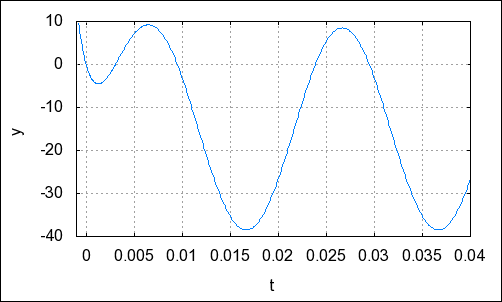
\includegraphics[width=9cm]{problema_2_6_img/problema_2_6_1.png}
\end{math}

\begin{math}\displaystyle
\parbox{8ex}{\color{labelcolor}(\%o64) }
$ $
\end{math}
%%%%%%%%%%%%%%%


\noindent
%%%%%%%%%%%%%%%
%%% INPUT:
\begin{minipage}[t]{8ex}{\color{red}\bf
\begin{verbatim}
-->  
\end{verbatim}}
\end{minipage}
\begin{minipage}[t]{\textwidth}{\color{blue}
\begin{verbatim}
kill(all);
\end{verbatim}}
\end{minipage}

\end{document}
